% \documentclass[handout]{beamer} %"handout" serveix per a treure els \pause
\documentclass{beamer} %"handout" serveix per a treure els \pause
\usepackage{preamble}

\usetheme{Copenhagen}
\usecolortheme{seahorse}

% \addbibresource{references.bib}

%gets rid of bottom navigation bars
\setbeamertemplate{footline}[frame number]{}

%gets rid of bottom navigation symbols
\setbeamertemplate{navigation symbols}{}

%gets rid of footer
%will override 'frame number' instruction above
%comment out to revert to previous/default definitions
\setbeamertemplate{footline}{}
% Remove the "Figure" prefix from captions
\captionsetup[figure]{labelformat=empty}
% \setbeameroption{show notes}


\title{Numerical propagation of errors\\of Earth-orbiting spacecraft}
\author{Víctor Ballester\texorpdfstring{\vspace{0.15cm}\\}{}{\small Supervisor: Josep Maria Mondelo}}
\institute{Departament de Matemàtiques\\Facultat de Ciències}
\titlegraphic{
\includegraphics[width=0.3\textwidth]{../Images/uab.pdf}}
\date{July 11, 2023}

\begin{document}
\frame{\titlepage}
\begin{frame}{Motivation}
  \begin{itemize}
    \item Around 7000 satellites (active and inactive) orbiting the Earth.
    \item Various unintentional collisions in the past.
    \item Point Earth model is not enough. We need a more accurate model.
  \end{itemize}
  \vspace{0.5cm}
  \textbf{Goal:}
  \begin{itemize}
    \item Develop a geopotential model of the Earth.
    \item Propagate the position of a satellite adding different perturbations.
    \item Estimate the error of the trajectory.
  \end{itemize}
\end{frame}
\begin{frame}{Equation for $V$}
  Let $\Omega\subseteq \RR^3$ be the region that occupies the Earth.
  \begin{gather*}
    \vf{g} = -\int_\Omega G\frac{\vf{r}-\vf{s}}{\norm{\vf{r}-\vf{s}}^3}\rho(\vf{s})\dd^3\vf{s}=\grad V\\
    V=\int_\Omega G\frac{\rho(\vf{s})}{\norm{\vf{r}-\vf{s}}}\dd^3\vf{s}
  \end{gather*}
  \begin{theorem}
    $V$ satisfies the following exterior boundary problem:\note{Comment the unicity of the solution}
    \begin{equation*}\label{eq:dirichletProblem}
      \begin{cases}
        \laplacian V = 0 & \text{in } \Omega^c    \\
        V = f            & \text{on } \Fr{\Omega} \\
        \displaystyle\lim_{\norm{\vf{r}}\to\infty}V=0
      \end{cases}
    \end{equation*}
    where $f:\Fr{\Omega}\to\RR$ is the gravitational potential on the surface of the Earth.
  \end{theorem}
\end{frame}
\begin{frame}
  Separation of variables: $V=R(r)\Theta(\theta)\Phi(\phi)$
  \begin{gather*}
    \begin{cases}
      \displaystyle\frac{{(r^2R')}'}{R}=n(n+1)                   \\
      \displaystyle\frac{1}{\Theta}\Theta''  =-m^2\vspace{0.1cm} \\
      \displaystyle\frac{\sin\phi}{\Phi}{(\sin\phi\Phi')}'+n(n+1){(\sin\phi)}^2  =m^2
    \end{cases}\!n,m\in\NN\cup\{0\}, m\leq n
  \end{gather*}
  Imposing boundary conditions:
  \begin{equation*}
    V =\frac{GM_\oplus}{R_\oplus}\sum_{n=0}^\infty \sum_{m=0}^n{\left(\frac{{R_\oplus}}{r}\right)}^{n+1}(\bar{C}_{n,m}Y_{n,m}^{\mathrm{c}}(\theta,\phi)+\bar{S}_{n,m}Y_{n,m}^{\mathrm{s}}(\theta,\phi))
  \end{equation*}
  where
  \begin{align*}
    Y_{n,m}^{\mathrm{c}}(\theta,\phi) & =N_{n,m}P_{n,m}(\cos\theta)\cos(m\phi) \\
    Y_{n,m}^{\mathrm{s}}(\theta,\phi) & =N_{n,m}P_{n,m}(\cos\theta)\sin(m\phi)
  \end{align*}
  are the \textbf{spherical harmonics}.
\end{frame}
\begin{frame}{Deviations of the Earth's rotation axis}
  \begin{minipage}{0.49\textwidth}
    \begin{figure}
      \centering
      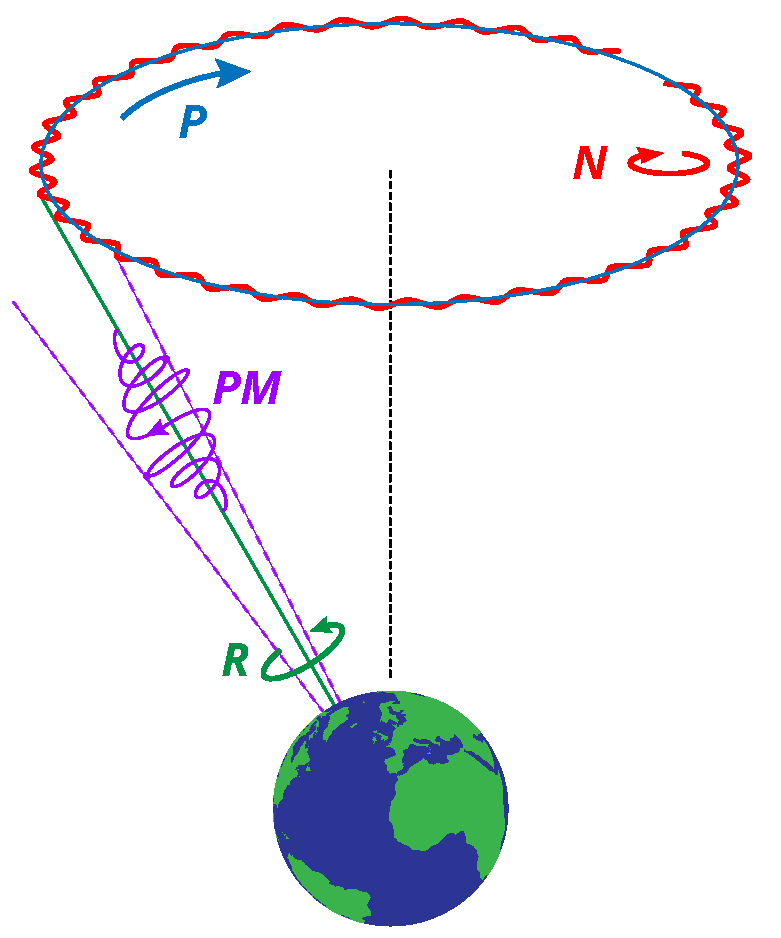
\includegraphics[width=\textwidth]{../Images/precession_nutation.pdf}
    \end{figure}
  \end{minipage}
  \begin{minipage}{0.49\textwidth}
    \begin{itemize}
      \item \textcolor[RGB]{0,113,188}{{Precession}}
      \item \textcolor[RGB]{255,0,0}{{Nutation}}
      \item \textcolor[RGB]{0,146,70}{{Rotation}}
      \item \textcolor[RGB]{158,0,255}{{Polar motion}}
    \end{itemize}
  \end{minipage}
\end{frame}
\begin{frame}{Inertial and non-inertial reference frames}
  \textbf{Quasi-inertial}:
  \begin{itemize}
    \item $x$-axis: pointing towards the $\overline{\Upsilon}$ of the J2000 date
    \item $z$-axis: perpendicular to the equator of the J2000 date
  \end{itemize}

  \textbf{Non-inertial} (Earth fixed):
  \begin{itemize}
    \item $x$-axis: pointing towards the zero meridian
    \item $z$-axis: perpendicular to the equator
  \end{itemize}

  In both systems $y$-axis is chosen in order to complete a right-handed system.
\end{frame}
\begin{frame}{Transformation between systems}



  \begin{figure}[htbp]
    \centering
    \begin{minipage}[ht]{0.3\textwidth}
      \centering
      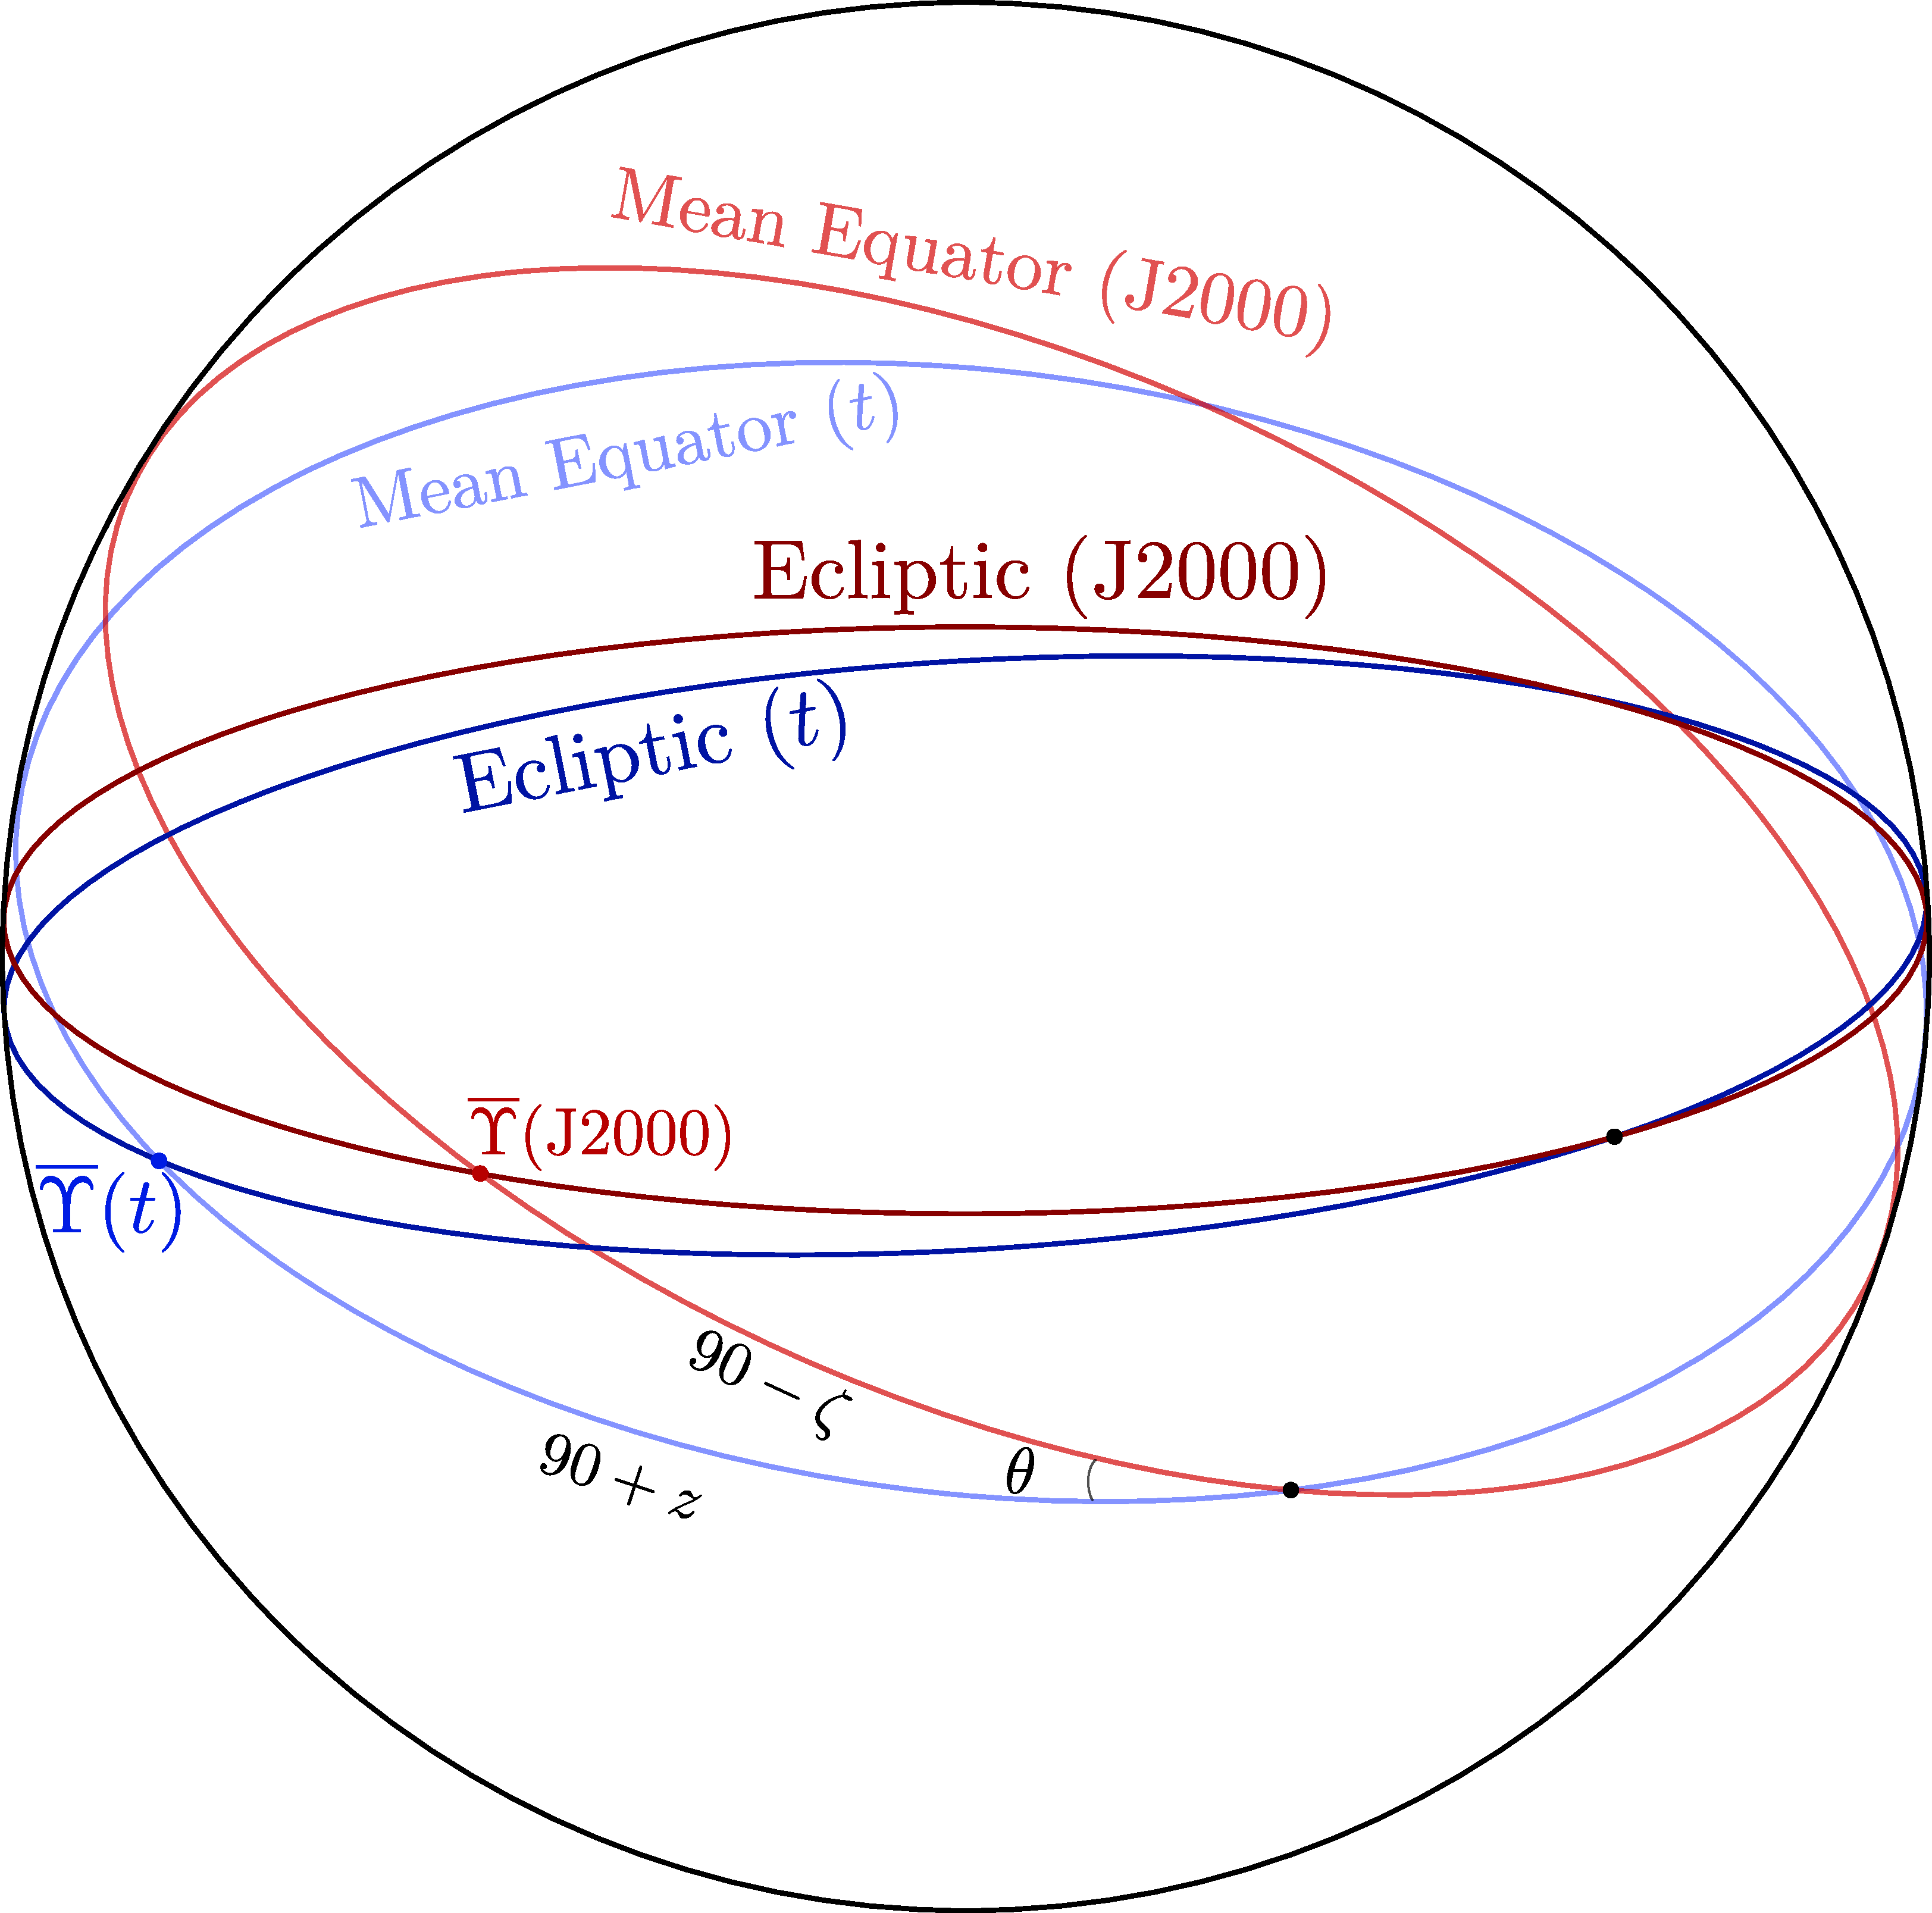
\includegraphics[width=\textwidth]{../Images/ecliptic_equator.pdf}
    \end{minipage}
    \hspace{0.025\textwidth}
    \begin{minipage}[ht]{0.3\textwidth}
      \centering
      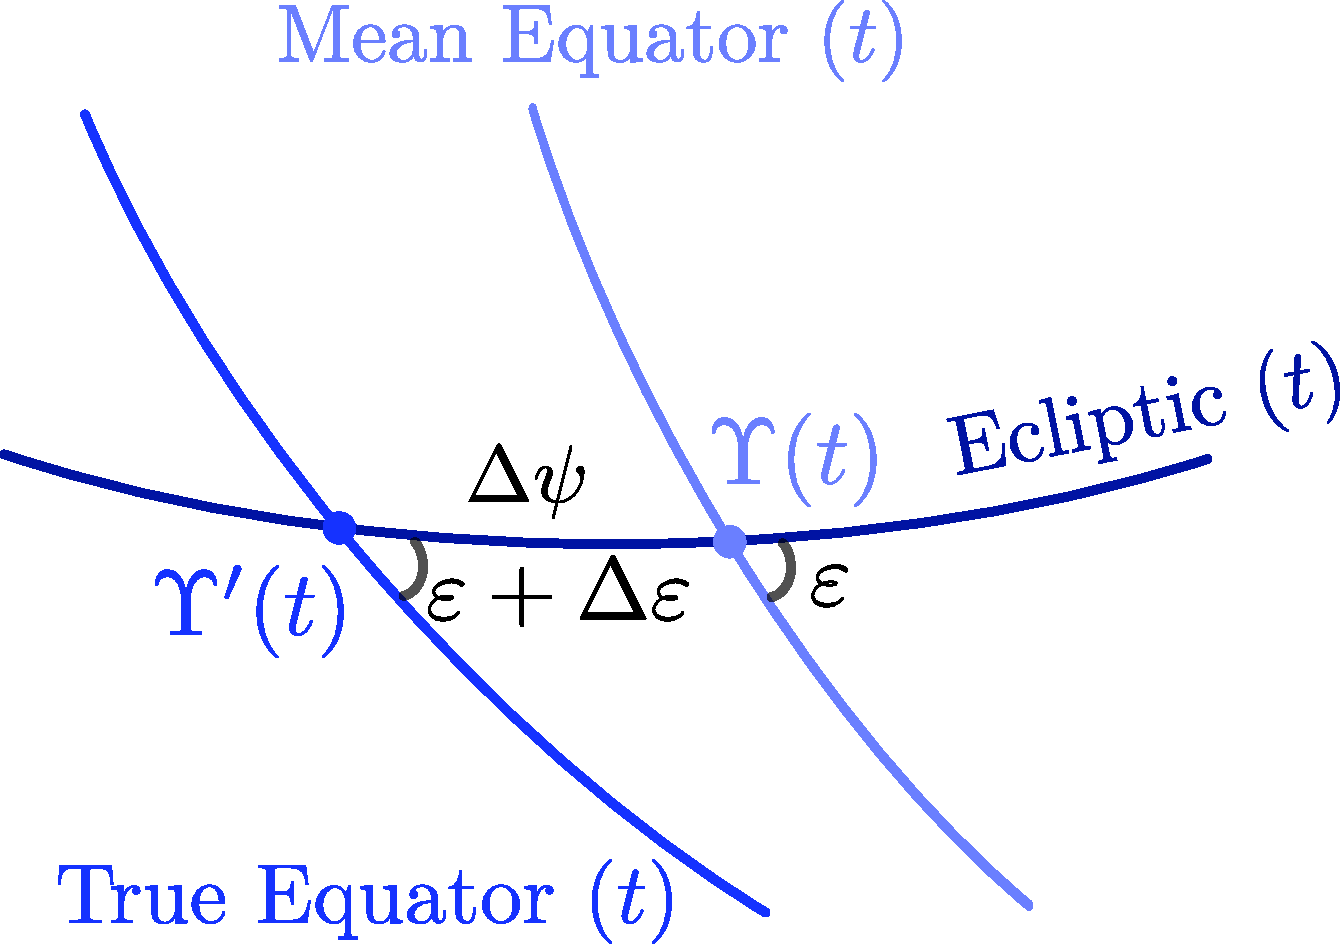
\includegraphics[width=0.9\textwidth]{../Images/nutation_matrix.pdf}
    \end{minipage}
    \hspace{0.025\textwidth}
    \begin{minipage}[ht]{0.3\textwidth}
      \centering
      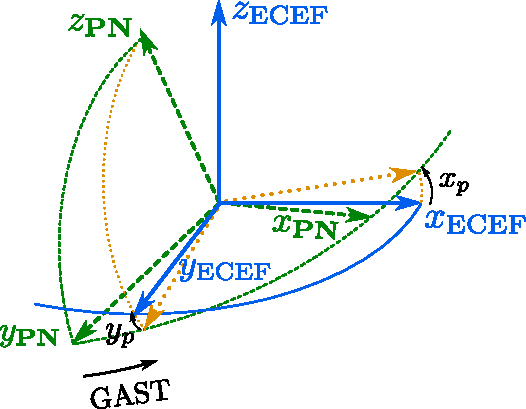
\includegraphics[width=0.9\textwidth]{../Images/polar_motion_matrix.pdf}
    \end{minipage}
  \end{figure}
\end{frame}
\begin{frame}
  \frametitle{Other perturbations}
  $\vf{r} = \text{satellite position with respect to Earth's center of mass}$

  \vspace{0.25cm}
  \begin{itemize}
    \item<1-> Third body perturbations (Moon and Sun): $$\frac{GM}{\norm{\vf{s}-\vf{r}}^2}(\vf{s}-\vf{r}) - \frac{GM}{\norm{\vf{s}}^2}\vf{s}$$
    \item<2-> Atmospheric drag: $$-\frac{1}{2}C_\mathrm{D} \frac{A}{m}\rho v_\mathrm{rel}\vf{v}_\mathrm{rel}$$
      where $\vf{v}_\mathrm{rel}=\dot{\vf{r}}-\vf{\omega}_\oplus\times\vf{r}$.
    \item<3-> Solar radiation pressure: $$
        -P_\odot C_\mathrm{R} \frac{A_\odot}{m} \frac{\vf{s}_\odot-\vf{r}}{\norm{\vf{s}_\odot-\vf{r}}}
      $$
  \end{itemize}
\end{frame}
\begin{frame}{Differential system}
  Using the Runge-Kutta-Fehlberg method of order 7(8) we will integrate the differential system:
  \begin{equation*}
    \begin{cases}
      \dot{\vf{r}}=\vf{v} \\
      \dot{\vf{v}}=\vf{a}_{\mathrm{GP}} + \delta_{\mathrm{D}}\vf{a}_{\mathrm{D}}+\delta_{\mathrm{R}}\vf{a}_{\mathrm{R}}+\delta_{\mathrm{sun}}\vf{a}_{\mathrm{sun}}+\delta_{\mathrm{moon}}\vf{a}_\mathrm{moon}
    \end{cases}
  \end{equation*}
  \pause
  \vspace{0.25cm}

  Initial conditions from \textbf{TLEs} (Two Line Elements sets).
  \begin{figure}
    \centering
    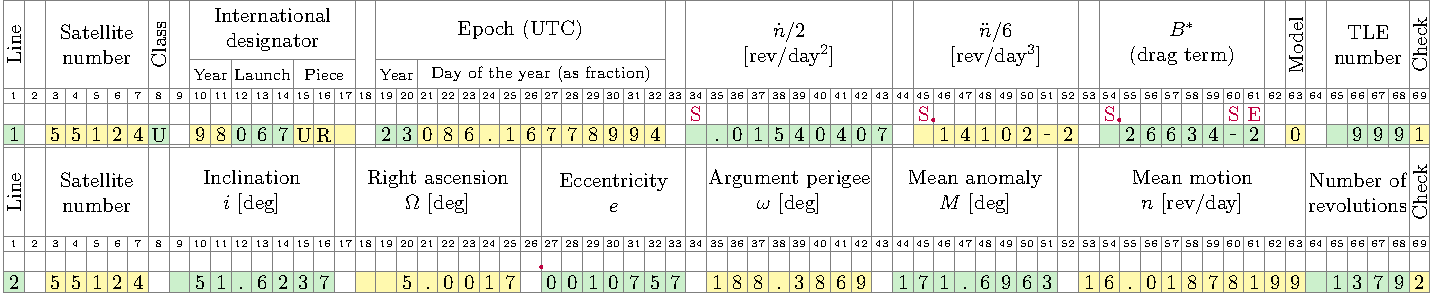
\includegraphics[width=\textwidth]{../Images/TLE.pdf}
  \end{figure}
\end{frame}
\begin{frame}{Results}
  Scheme of our simulation:
  \begin{figure}
    \centering
    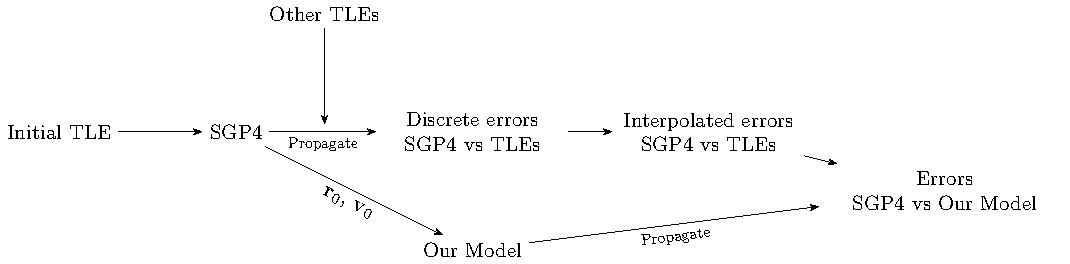
\includegraphics[width=\textwidth]{../Images/simulation_scheme.pdf}
  \end{figure}
  \begin{minipage}{0.4\textwidth}
    \begin{figure}[ht]
      \centering
      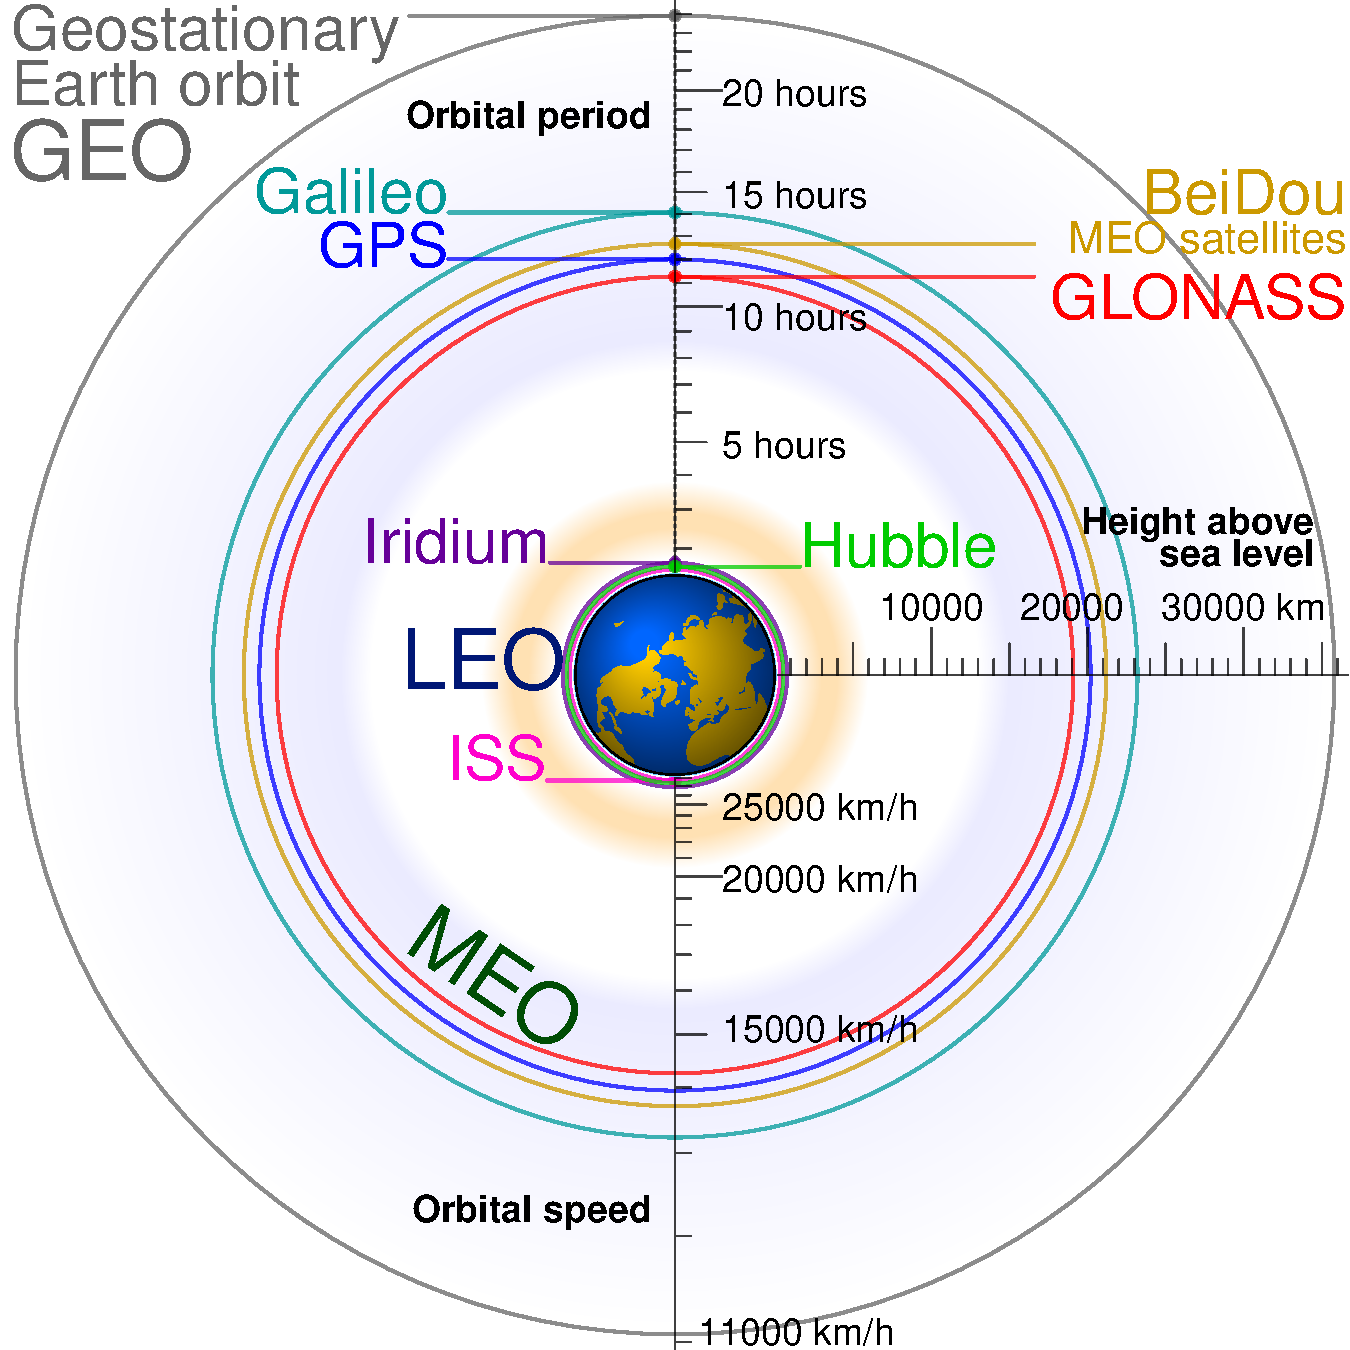
\includegraphics[width=\textwidth]{../Images/satellite_orbits_custom.pdf}
    \end{figure}
  \end{minipage}\hfill
  \begin{minipage}{0.55\textwidth}
    Zones that we will explore:
    \begin{itemize}
      \item \textbf{L}ow \textbf{E}arth \textbf{O}rbit satellites
      \item \textbf{M}edium \textbf{E}arth \textbf{O}rbit satellites
      \item \textbf{G}eostationary \textbf{E}arth \textbf{O}rbit satellites
    \end{itemize}
  \end{minipage}
\end{frame}
\begin{frame}{Results - LEO}
  \begin{itemize}
    \item ISS makes $\sim 16$ orbits per day.
    \item LEO satellites interact with the atmosphere.
    \item The atmospheric drag is difficult to predict.
  \end{itemize}
  \begin{figure}[htbp]
    \centering
    \begin{minipage}[ht]{0.45\textwidth}
      \centering
      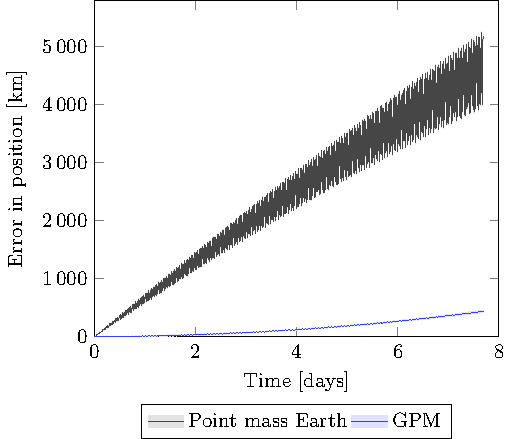
\includegraphics[width=\textwidth]{../Images/simulation/ISS_pointMass_comparison.pdf}
      \caption{\hspace{0.8cm}ISS}
    \end{minipage}
    \hspace{0.0333333\textwidth}
    \begin{minipage}[ht]{0.45\textwidth}
      \centering
      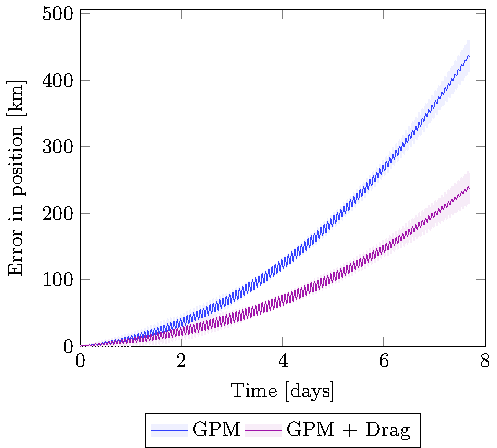
\includegraphics[width=\textwidth]{../Images/simulation/ISS.pdf}
      \caption{\hspace{0.8cm}ISS}
    \end{minipage}
  \end{figure}
\end{frame}
\begin{frame}{Results - MEO}
  \begin{figure}[ht]
    \centering
    \begin{minipage}[ht]{0.45\textwidth}
      \centering
      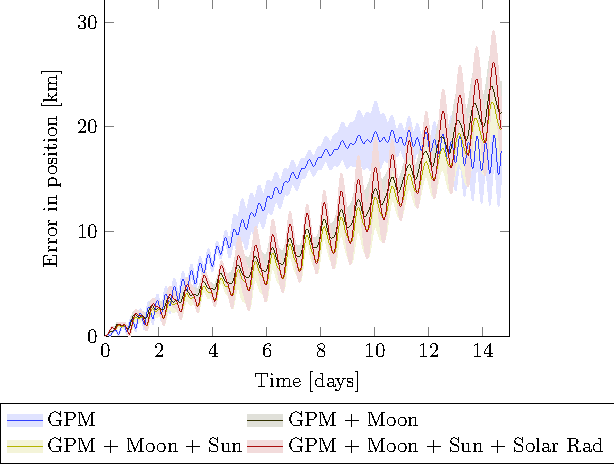
\includegraphics[width=\textwidth]{../Images/simulation/SIRIUS.pdf}
      \caption{Sirius-3}
    \end{minipage}
    \hspace{0.0333333\textwidth}
    \begin{minipage}[ht]{0.45\textwidth}
      \centering
      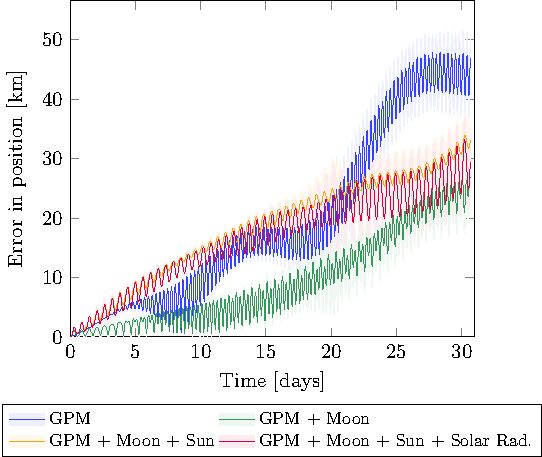
\includegraphics[width=\textwidth]{../Images/simulation/GALILEO.pdf}
      \caption{Galileo-20}
    \end{minipage}
  \end{figure}
  \begin{itemize}
    \item GPM is very oscillatory.
    \item Sun and Moon reduce the oscillations.
    \item Solar radiation increases the oscillations.
  \end{itemize}
\end{frame}
\begin{frame}{Results - GEO}
  \begin{minipage}{0.48\textwidth}
    \begin{figure}[ht]
      \centering
      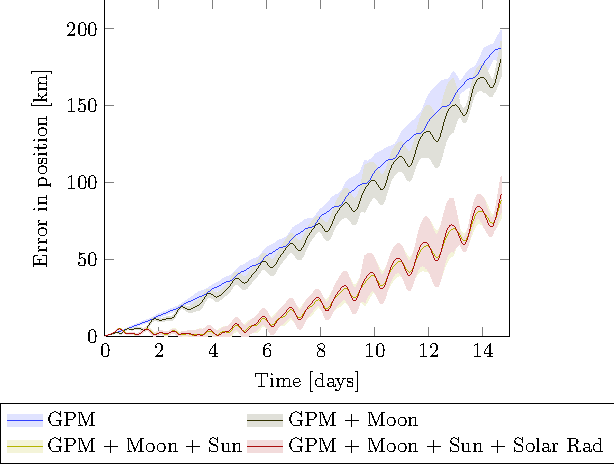
\includegraphics[width=\textwidth]{../Images/simulation/TDRS-3.pdf}
      \caption{TDRS-3}
    \end{figure}
  \end{minipage}
  \hfill
  \begin{minipage}{0.48\textwidth}
    \begin{itemize}
      \item Adding the Sun and the Moon the errors are reduced.
      \item Solar radiation again increases the oscillations.
      \item Maneuver at around the 13th day.
    \end{itemize}
  \end{minipage}
\end{frame}
\begin{frame}{Conclusions}
  \begin{itemize}
    \item The point mass model is not enough to predict the orbit of a satellite.
    \item Adding both together the Sun and the Moon the variability of the errors is reduced.
    \item Radiation pressure increases the oscillations.
  \end{itemize}
  \textbf{Improvements:}
  \begin{itemize}
    \item Atmospheric drag and solar radiation bad modelled.
    \item Study the influence of the inclination and eccentricity on the errors.
  \end{itemize}
\end{frame}
\end{document}